\documentclass{report}
\renewcommand{\baselinestretch}{1.5} 
\usepackage{amsmath}
\usepackage{amssymb}
\usepackage{tikz}
\usepackage{natbib}
\usepackage[margin=1in]{geometry}
\begin{document}
\begin{Large}
\begin{center}
\Large{Masoud Jabbari \ \ \ \ \  Empirical Methods \ \ \ \ \ \ Set\#2}
\end{center}
\end{Large}

In all questions I add $Q$ and the number of the question to the variables, so for example $XQ1$ is the variable $X$ defined in question 1. 


Q1.

By simply substituting $\nu_A=\nu_B=2$ and $p_A=p_B=1$ in consumer demand we would have
\begin{equation*}
D_A=\frac{exp(1)}{1+exp(1)+exp(1)}=\frac{e}{1+2\times e}
\end{equation*}
\begin{equation*}
D_B=\frac{exp(1)}{1+exp(1)+exp(1)}=\frac{e}{1+2\times e}
\end{equation*}
\begin{equation*}
D_0=\frac{1}{1+exp(1)+exp(1)}=\frac{1}{1+2\times e}
\end{equation*}

Q2.
Firm $A$ solves
\begin{equation*}
\max_{p_{A}}p_{A}D_{A}
\end{equation*}
By writing first order conditions we have:
\begin{equation*}
D_{A}+p_{A}\times\left[-D_{A}\left(1-D_{A}\right)\right]=D_{A}-p_{A}\times D_{A}+p_{A}\times D_{A}^2=0\Rightarrow 1-p_{A}+p_{A}D_{A}=0 
\end{equation*}
So by substituting $v_{A}=v_{B}=2$ and doing some simple algebra we have:
\begin{equation}
\left(1-p_{A} \right)\left(1+e^{2-p_{B}}\right)+e^{2-p_{	A}}=0  
\end{equation}
The problem for firm B is symmetric, so we have:
\begin{equation}
\left(1-p_{B} \right)\left(1+e^{2-p_{A}}\right)+e^{2-p_{B}}=0  
\end{equation}
Now we should solve the system of equations $1$ and $2$ to find Bertnard equilibrium prices. Because of the hint that the equilibrium is unique and also due to symmetry the guess is that the equilibrium should be of the type $p_{A}=p_{B}$, but since the problem asks to solve with Broyden's method, I do not use this guess to keep the multidimensional aspect of this method. 
I used $P_{A}=P_{B}=1.5$ as initial guess and $1e^{-6}$ as tolerance. The codes are attached. By solving the non-linear system the Bertrand equilibrium prices are $P_{A}=P_{B}=1.5989$ and the equilibrium quantities are $D_{A}=D_{B}=0.3746, D_{0}=0.2508$. The code converged after 4 iterations and the convergence time in my system was 0.008447 seconds.

Q3. Similar to question 2 and by using Gauss-Sidel method with secant for Jacobian, I solved the Bertrand equilibrium. I used $P_{A}=P_{B}=1.5$ as initial guess and $1e^{-6}$ as tolerance. The codes are attached. By solving the non-linear system the Bertrand equilibrium prices are $P_{A}=P_{B}=1.5989$ and the equilibrium quantities are $D_{A}=D_{B}=0.3746, D_{0}=0.2508$. The code converged after 14 iterations and the convergence time in my system was   0.005304 seconds. This method was faster, and the reason I think is that it uses immediately from the new component and updated information. 

Q4. I used the updating rule of $P^{t+1}=\frac{1}{1-D(P^{t})}$. I solved the Bertrand equilibrium. I used $P_{A}=P_{B}=1.5$ as initial guess and $1e^{-6}$ as tolerance. The codes are attached. By solving the non-linear system the Bertrand equilibrium prices are $P_{A}=P_{B}=1.5989$ and the equilibrium quantities are $D_{A}=D_{B}=0.3746, D_{0}=0.2508$. The code converged after 10 iterations and the convergence time in my system was  0.006996 seconds. This method was faster than first one but slower than second one. Actually, in different runs I got different times for solving the equilibrium!

Q5. 
 I use Gauus-Sidel method and find equilibrium prices for product A and product B, when quality of product A is fixed at 2 and the quality of product B varies in the range 0 to 3. As prediction, the equilibrium price for product B increases with increasing in the quality of it, and the equilibrium price for product A, as the quality of product B increses. Figure 1 displays this. 
 \begin{figure}
 \centering
 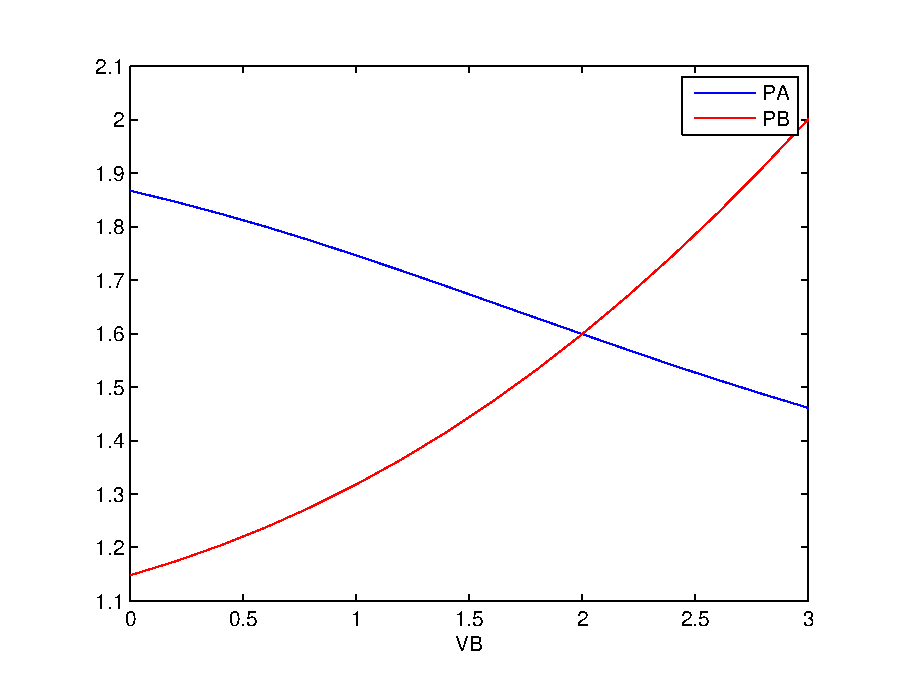
\includegraphics[width=0.75\textwidth]{FIGQ5}
 \caption{The effect of Product B quality on Product A and Product B prices}\label{figq1}
 \end{figure}











\end{document}
